\documentclass[a4paper,12pt]{article}
\usepackage{cmap}
\usepackage[utf8]{inputenc}
\usepackage[russian]{babel}

\usepackage{amsmath}
\usepackage[left=2cm,right=2cm,top=3cm,bottom=2cm]{geometry}
\usepackage[dvips]{graphicx}
\graphicspath{{\noiseimages}}
\usepackage{graphicx}

\headheight16pt

\usepackage{indentfirst}

\usepackage{fancyhdr}
\pagestyle{fancy}
\fancyhead{}
\fancyhead[LO]{Межрегиональная физическая олимпиада 2013---2014. Заочный тур}
\fancyhead[RO]{Стр.~\thepage~из 3}
\fancyfoot{}

\newcommand\hr[1]{\left({#1}\right)}
\newcommand\un[1]{\,\emph{#1}}

\def\thesection{\arabic{section}.}
\def\thesubsection{\arabic{section}.\arabic{subsection}.}

\begin{document}

\section{Теоретические задачи}

\subsection{Кто быстрее?}
Сева везет Никиту на санках по горизонтальной дороге. По дороге Никита стал спорить с~Севой,
что он, находясь на санках, которые везет Сева, может двигаться быстрее него, пассивно сидя
на санках и~никак не способствуя этому движению (не отталкиваясь ногами, не вытягивая
веревку~и\,т.\,д.). Может ли Никита быть прав?

\subsection{Тепло и~диод} На рис.~1 представлена вольт-амперная характеристика диода.
Какое количество теплоты выделится на этом диоде за~$12$~секунд, если в~течение этого
времени менять напряжение с~$0$ до~$ 1,5$\un{В}?

\medskip
\centerline{\includegraphics[width=0.5\linewidth]{VCP21}}
\medskip
\centerline{\small Рис.~1}

\subsection{Тележка Жени}
Женя соорудила тележку, изображённую на рис.~2. Колёса тележки сделаны из катушек
(цилиндры с~широкой кромкой). Радиусы цилиндров~---~$r$, радиусы кромок~---~$kr$.
На цилиндрах лежит ещё одно колесо, на которое Женя кладёт линейку и~тянет на себя
со скоростью~$v$. Какой при этом будет скорость тележки? Колёса не проскальзывают
относительно поверхности, друг друга и~линейки. Также опишите качественно,
что будет происходить при $k = 1$ (то есть в~случае, когда кромки отсутствуют).

\medskip
\centerline{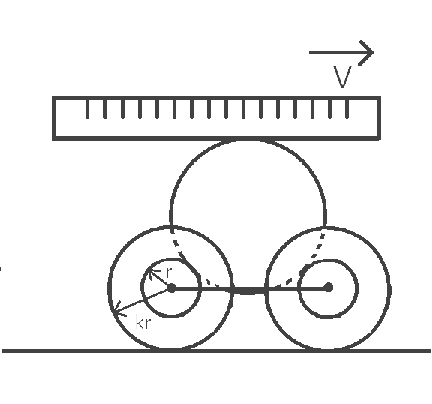
\includegraphics[width=0.3\linewidth]{T}}
\medskip
\centerline{\small Рис.~2}

\newpage

\subsection{Кирпич и~песок}
Есть два одинаковых цилиндрических теплоизолированных сосуда с~одним молем идеального одноатомного газа
при комнатной температуре, находящимся под поршнем массы~$1$\un{кг} (снаружи вакуум). На первый поршень
резко положили кирпич массой~$1$\un{кг}, а~на второй аккуратно клали по песчинке до тех пор, пока масса
песка на поршне не достигла~$1$\un{кг}. Для каждого из поршней найдите положение равновесия. Что будет
происходить с~каждым из~поршней? В~чём различие между этими двумя ситуациями?


\subsection{Солнечные очки}
Бывают солнечные очки, которые с~внешней стороны кажутся зеркальными, а~с~внутренней стороны,
естественно, через них можно смотреть как через обычные очки. Интересное явление состоит в~том,
что если их перевернуть (смотреть снаружи), то почти ничего не видно, то есть стекло является
принципиально асимметричным. Подумайте, как могут быть устроены такие очки?

\section{Экспериментальные задачи}

\subsection{Притяжение и~отталкивание}

Известно, что плавающие в~блюдце с~водой небольшие предметы, например спички или канцелярские скрепки,
<<притягиваются>>. А~могут ли такие мелкие предметы, плавая на поверхности жидкости,
отталкиваться? Если да, поставьте эксперимент, демонстрирующий это.

\subsection{Капли, скатывающиеся с~зеркала}
Наблюдая за каплями, скатывающимися с~наклонного зеркала, Петя заметил, что капли не~скатываются,
если они меньше определенного размера. Попробуйте экспериментально получить зависимость минимальной
массы скатывающейся капли от угла наклона зеркала.

\subsection{Вращательный маятник}
Если какой-либо груз подвесить на верёвке или нити, то можно будет наблюдать колебания:
если немного закрутить груз, он будет вращаться попеременно то~в~одну, то~в~другую сторону.
Период этих колебаний зависит от длины и~материала нити, от массы, формы груза и~даже его положения.
В~частности, если подвесить один и~тот же груз на одной и~той же нити за разные точки, могут
получиться разные периоды. Экспериментально найдите отношения этих периодов:
\begin{enumerate}
\item Для диска, подвешенного за край и~за центр.
\item Для куба, подвешенного за середину грани, и~куба, подвешенного за вершину.
\end{enumerate}

\subsection{Электрофрукт}
Известно, что при помощи двух предметов из разных металлов, воткнутых в~лимон или яблоко, можно получить~ЭДС.
\begin{enumerate}
 \item Измерьте внутреннее сопротивление <<фруктовой батарейки>>.

 \item Подключите к~вашей  <<фруктовой батарейке>> обычную и~измерьте сопротивление на том же участке,
 что и~в предыдущем пункте. Что изменилось? Попробуйте объяснить результат.

 \item Как зависит общая энергия, которую можно получить, от массы фрукта? Имеется в~виду зависимость
 от массы для какого-то одного, выбранного вами фрукта, с~одним типом электродов.
\end{enumerate}

\subsection{$S$-образная трубка}
В своей книжке <<Вы, конечно же, шутите, мистер Фейнман>> (``Surely you are joking, Mr~Feynman'')
известный физик Ричард Фейнман приводит следующую задачу:
\begin{quote} Имеется $S$-образный разбрызгиватель для лужаек~--- $S$-образная труба на оси;
вода бьёт струей под прямым углом к~оси и~заставляет трубу вращаться в~определенном направлении.
Каждый знает, куда она вертится~--- трубка убегает от уходящей воды. Вопрос стоит так: пусть у~вас
есть озеро или плавательный бассейн, то есть большой запас воды. Вы помещаете разбрызгиватель целиком
под воду и~начинаете всасывать воду вместо того, чтобы разбрызгивать ее струей. В~каком направлении
будет поворачиваться трубка?
\end{quote}
Далее он приводит два варианта решения, приводящих к~противоречащим друг другу результатам:
\begin{quote}
Я приведу вам аргумент, который заставляет думать так, и~другой аргумент, заставляющий думать наоборот. Хорошо?
Одно соображение состоит в~том, что, когда вы всасываете воду, она как бы втягивается в~сопло.
Поэтому трубка подается вперед, по направлению к~входящей воде.
Но вот приходит кто-то другой и~говорит: <<Предположим, что мы удерживаем устройство в~покое и~спрашиваем,
какой момент вращения для этого необходим. Мы все знаем, что, когда вода вытекает, трубку приходится
держать с~внешней стороны $S$-образной кривой~--- из-за центробежной силы воды, проходящей по контуру.
\hbox{Ну~а~если} вода идет по~той~же кривой в~обратном направлении, центробежная сила остается той же
и~направлена в~сторону внешней части кривой. Поэтому оба случая одинаковы, и~разбрызгиватель
будет поворачиваться в~одну и~ту~же сторону вне зависимости от~того, выплескивается ли вода
струей или всасывается внутрь>>.
\end{quote}
Попробуйте найти все ошибки в~этих рассуждениях и~проверьте экспериментально,
в~какую сторону на самом деле вращается трубка.

\end{document}
